\documentclass[tikz,border=2pt]{standalone}
\usepackage{amsmath}
\usetikzlibrary{arrows.meta}
\begin{document}
% FIFO single server, A = (1,2,5,9,10), S = (3,2,1,2,2): start of service max{A_k, D_{k-1}},
% departures D = (4,6,7,11,13), waits W = (0,2,1,0,1); dotted lines carry D_{k-1} to row k.
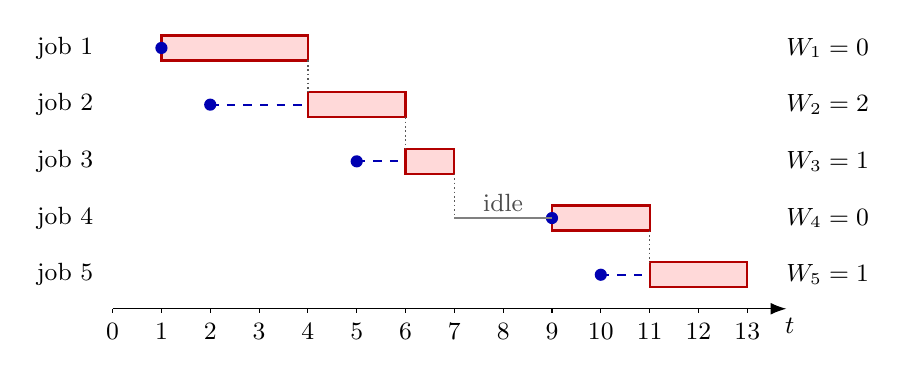
\begin{tikzpicture}[font=\small, >={Latex[length=2mm]}, x=0.62cm, y=0.72cm]
  % rows: job k at height 5-k
  \foreach \k/\a/\s/\d/\w in {1/1/1/4/0, 2/2/4/6/2, 3/5/6/7/1, 4/9/9/11/0, 5/10/11/13/1} {
    \pgfmathsetmacro{\y}{5-\k}
    \node[anchor=east] at (-0.2,\y) {job \k};
    \ifnum\a<\s
      \draw[blue!70!black, thick, dashed] (\a,\y) -- (\s,\y);
    \fi
    \filldraw[red!70!black, fill=red!15, thick] (\s,\y-0.22) rectangle (\d,\y+0.22);
    \fill[blue!70!black] (\a,\y) circle (2.2pt);
    \node[anchor=west] at (13.6,\y) {$W_{\k}=\w$};
  }
  % predecessor departures carried down to the next row
  \foreach \x/\ytop/\ybot in {4/3.78/3.22, 6/2.78/2.22, 7/1.78/1, 11/0.78/0.22} {
    \draw[gray!70!black, semithick, densely dotted] (\x,\ytop) -- (\x,\ybot);
  }
  \draw[gray, thin] (7,1) -- (9,1);
  \node[gray!60!black, anchor=south, inner sep=2pt] at (8,1) {idle};
  % time axis
  \draw[->] (0,-0.6) -- (13.8,-0.6) node[anchor=north west, xshift=-4pt] {$t$};
  \foreach \t in {0,1,...,13} \draw (\t,-0.6) -- (\t,-0.68) node[below] {$\t$};
\end{tikzpicture}
\end{document}
